\documentclass[a4paper,10pt]{article}

\usepackage{amsmath}
\usepackage[latin1]{inputenc}
\usepackage{fontenc}
\usepackage{graphicx,color}
\DeclareGraphicsRule{.pdftex}{pdf}{*}{}
\usepackage{wasysym}
\usepackage{tikz} %For directory tree on code in appendix
\usepackage{url}

\newcommand{\nucl}[3]{
\ensuremath{
\phantom{\ensuremath{^{#1}_{#2}}}
\llap{\ensuremath{^{#1}}}
\llap{\ensuremath{_{\rule{0pt}{.75em}#2}}}
\mbox{#3}
}
}

\makeatletter
\newcount\dirtree@lvl
\newcount\dirtree@plvl
\newcount\dirtree@clvl
\def\dirtree@growth{%
  \ifnum\tikznumberofcurrentchild=1\relax
  \global\advance\dirtree@plvl by 1
  \expandafter\xdef\csname dirtree@p@\the\dirtree@plvl\endcsname{\the\dirtree@lvl}
  \fi
  \global\advance\dirtree@lvl by 1\relax
  \dirtree@clvl=\dirtree@lvl
  \advance\dirtree@clvl by -\csname dirtree@p@\the\dirtree@plvl\endcsname
  \pgf@xa=0.7cm\relax
  \pgf@ya=-0.5cm\relax
  \pgf@ya=\dirtree@clvl\pgf@ya
  \pgftransformshift{\pgfqpoint{\the\pgf@xa}{\the\pgf@ya}}%
  \ifnum\tikznumberofcurrentchild=\tikznumberofchildren
  \global\advance\dirtree@plvl by -1
  \fi
}

\tikzset{
  dirtree/.style={
    growth function=\dirtree@growth,
    every node/.style={anchor=north},
    every child node/.style={anchor=west},
    edge from parent path={(\tikzparentnode\tikzparentanchor) |- (\tikzchildnode\tikzchildanchor)}
  }
}
\makeatother


\usepackage[nottoc,numbib]{tocbibind}
\title{Answers to Homework II}
\author{Petter S\"{a}terskog\footnote{petter.saterskog@gmail.com}}
\date{\today}

\begin{document}

\maketitle

%\begin{figure}
%centering
%\includegraphics[width=11cm]{cms-crop.pdf}
%\caption{FLUKA simulation of the flux spectrum in CMS-UXC at the position of our detectors.}
%\label{f:cmsPhi}
%\end{figure}
\section{Question 3}
\subsection{Q1}
I downloaded the data from \url{http://hepdata.cedar.ac.uk/pdf/pdf3.html}. I used group CTEQ45 and set cteq5m. I used $Q^2=100 \mathrm{GeV}^2$. I chose particle type all to get PDFs for $u, \bar{u}, d, \bar{d}, s, c, b, g$. The site did not have information on $\bar{s}, \bar{c}, \bar{b}$ so I assume they have the same PDFs as their antiparticles. Virtual particles are created in particle-antiparticle pairs. The PDFs, $f(x,Q^2)$, were given as $g(x,Q^2)=xf(x,Q^2)$. Integrating these functions gives the mean energy fraction for that particle type.
\begin{equation}
 \frac{E_i}{E_{proton}}=\int_0^1xf_i(x,Q^2)\mathrm{d}x=\int_0^1g_i(x,Q^2)\mathrm{d}x
\end{equation}
This has been calculated numerically and the result is seen in Table \ref{q100}.\\
Integrating $f_i(x,Q^2)$ gives the number of particle $i$ present in the proton. But this diverges in the low energy limit. What can be calculated instead is the asymetry in number between particle and antiparticle.
\begin{equation}
 n_i=\int_0^1x(g_i(x,Q^2)-g_{\bar{i}}(x,Q^2))\mathrm{d}x
\end{equation}
This is 0 by assumption for $s, c, b$ but not for $u, d$. This has been calculated numerically and the result is seen in Table \ref{q100}. The total charge and energy has been calculated using this and the result is seen in Table \ref{q100}.
\begin{table}[ht]
\caption{Results for $Q^2=100 \mathrm{GeV}^2$}
\label{q100}
\centering % used for centering table
\begin{tabular}{cccc} % centered columns (4 columns)
\hline
Parton & t asymmetry & Charge contribution & Energy contribution\\
\hline
$u$ & 1.9993 & 1.3329 & 0.2601 \\
$d$ & 1.0059 & -0.3353 & 0.1308 \\
$\bar{u}$ & - & - & 0.0323\\
$\bar{d}$ & - & - & 0.0392\\
$s, \bar{s}$ & - & - & 0.0249\\
$c, \bar{c}$ & - & - & 0.0147\\
$b, \bar{b}$ & - & - & 0.0049\\
$g$ & - & - & 0.4615\\
Total & 3.0052 & 0.9976 & 1.0129
\end{tabular}
\end{table}
\subsection{Q2}
I varied the value of $Q^2$ and the results are seen in Table \ref{q0.001}, \ref{q1}, \ref{q100}, \ref{q10000}. The results are the same but the precision of the numerical integral goes down as the PDFs become more peaked at lower energy for the high $Q^2$-values.
 \begin{table}[ht]
\caption{Results for $Q^2=0.001 \mathrm{GeV}^2$}
\label{q0.001}
\centering % used for centering table
\begin{tabular}{cccc} % centered columns (4 columns)
\hline
Parton & t asymmetry & Charge contribution & Energy contribution\\
\hline
$u$ & 1.9999 & 1.3332 & 0.3791 \\
$d$ & 1.0004 & -0.3335 & 0.1769 \\
$\bar{u}$ & - & - & 0.0229\\
$\bar{d}$ & - & - & 0.0337\\
$s, \bar{s}$ & - & - & 0.0113\\
$c, \bar{c}$ & - & - & 0.0000\\
$b, \bar{b}$ & - & - & 0.0000\\
$g$ & - & - & 0.3654\\
Total & 3.0003 & 0.9998 & 1.0006
\end{tabular}
\end{table}


 \begin{table}[ht]
\caption{Results for $Q^2=1 \mathrm{GeV}^2$}
\label{q1}
\centering % used for centering table
\begin{tabular}{cccc} % centered columns (4 columns)
\hline
Parton & t asymmetry & Charge contribution & Energy contribution\\
\hline
$u$ & 1.9999 & 1.3332 & 0.3791 \\
$d$ & 1.0004 & -0.3335 & 0.1769 \\
$\bar{u}$ & - & - & 0.0229\\
$\bar{d}$ & - & - & 0.0337\\
$s, \bar{s}$ & - & - & 0.0113\\
$c, \bar{c}$ & - & - & 0.0000\\
$b, \bar{b}$ & - & - & 0.0000\\
$g$ & - & - & 0.3654\\
Total & 3.0003 & 0.9998 & 1.0006
\end{tabular}
\end{table}

 \begin{table}[ht]
\caption{Results for $Q^2=10000 \mathrm{GeV}^2$}
\label{q10000}
\centering % used for centering table
\begin{tabular}{cccc} % centered columns (4 columns)
\hline
Parton & t asymmetry & Charge contribution & Energy contribution\\
\hline
$u$ & 1.9991 & 1.3327 & 0.2210 \\
$d$ & 0.9997 & -0.3332 & 0.1151 \\
$\bar{u}$ & - & - & 0.0356\\
$\bar{d}$ & - & - & 0.0412\\
$s, \bar{s}$ & - & - & 0.0295\\
$c, \bar{c}$ & - & - & 0.0213\\
$b, \bar{b}$ & - & - & 0.0132\\
$g$ & - & - & 0.4763\\
Total & 2.9988 & 0.9995 & 1.0173
\end{tabular}
\end{table}
\subsection{Q3}
The antiproton is the antiparticle to the proton. The PDFs are the same but for the antiparticles of the partons. So the $u$ PDF is that of $\bar{u}$ and so on.\\
The $u$ and $d$-quarks have similar masses and the electromagnetic interaction is weak compared to the strong interaction which is isospin invariant. $u, \bar{u}$ and $d, \bar{d}$ can then be interchanged assuming isospin invariance and the neutron PDFs are obtained.
\section{Question 4}
The integral in the handwritten notes has been calculated numerically for different invariant masses and proton-proton center of mass energy. The result is seen in Figure \ref{cc}.
\begin{figure}
\centering
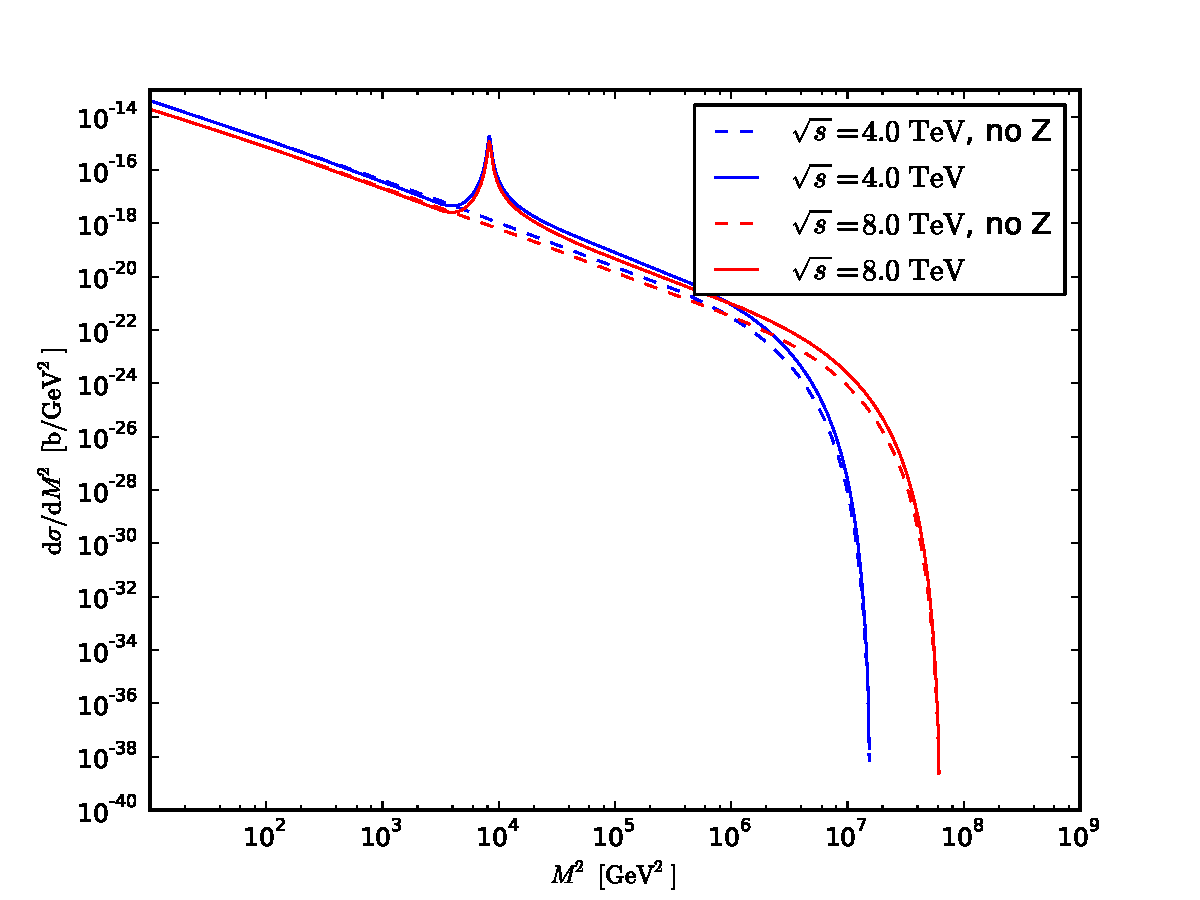
\includegraphics[width=11cm]{../cc.pdf}
\caption{Differential cross-section calculated by numerical integration.}
\label{cc}
\end{figure}

\end{document}
